\chapter{ShallWeGo}
\newenvironment{code}{\captionsetup{type=listing}}{}

\begin{citazione}
    \textit{Lo scopo di questo capitolo è di descrivere in termini di implementazione il funzionamento e l'architettura della piattaforma. In particolare, si focalizza l'attenzione sulle tecnologie utilizzate per lo sviluppo del server e del client della piattaforma, oltre che ad altre tecnologie impiegate per il corretto funzionamento delle componenti.}
\end{citazione}

\newpage

\section{Requisiti funzionali}
    Allo scopo di questo lavoro di tesi, le seguenti funzionalità visibili all'utente sono state implementate:

    \begin{itemize}
        \item L'utente può visualizzare tramite una mappa le fermate del trasporto pubblico presenti nin una determinata zona ed ottenerne i dettagli;
        \item Allo stesso modo, l'utente può visualizzare gli eventi temporanei in una determinata zona ed ottenerne i dettagli;
        \item L'utente può aggiungere delle fermate ad un elenco di fermate preferite;
        \item L'utente può visualizzare i dettagli e le destinazioni di una linea di trasporto pubblico;
        \item L'utente può seguire in diretta su una mappa l'andamento di una corsa e visualizzarne i dettagli;
        \item L'utente può segnalare l'affollamento di una fermata;
        \item L'utente può segnalare l'affollamento di una corsa;
        \item L'utente può segnalare la presenza di una fermata in un punto preciso sulla mappa o rapidamente presso la propria posizione;
        \item L'utente può segnalare la presenza di un'azienda di trasporto;
        \item L'utente può aggiungere una linea di trasporto pubblico ad un'azienda;
        \item L'utente può verificare, se gli sono state assegnate, tutti i tipi di segnalazioni appena descritti.
        \item L'utente può effettuare una segnalazione di un evento temporaneo in un punto preciso della mappa o rapidamente presso la propria posizione.
        \item L'utente può fornire aggiornamenti sulla propria posizione nell'ambito di una corsa espletata da una linea di trasporto pubblico e condividerne i dettagli.
    \end{itemize}

\section{Architettura del sistema}
    Il sistema ShallWeGo si configura come una classica architettura \textbf{client-server}.
    \begin{itemize}
        \item Il server consiste \textit{Java Enterprise application}, che accetta connessioni dal client sotto forma di richieste ad API REST.
        \item Il client è stato realizzato tramite un'applicazione utilizzabile sulla piattaforma Android dalla versione 10 in poi, a causa di scelte implementative riguardo alcune librerie incluse nel progetto. Queste scelte saranno documentate più avanti nel capitolo.
    \end{itemize}

    Per quanto riguarda la parte server, essa risulta composta da due macrocomponenti:

    \begin{itemize}
        \item La Java Application già accennata
        \item La componente che ospita la logica ed il database utilizzato da Nominatim, che è dislocato su un'altra macchina che viene utilizzata solo per questo scopo.
    \end{itemize}

\section{ShallWeGo: Il Server}
    Il server, come precedentemente menzionato, è realizzato usando le specifiche Java Enterprise Edition (da qui in poi \textit{Java EE}), usando a questo scopo il framework \textbf{\textit{Spring Boot}}, che permette una più semplice realizzazione dei task necessari a sviluppare un'applicazione che sfrutta il paradigma Client-Server, come ad esempio la gestione delle API accessibili dall'esterno i cosiddetti \textit{endpoint} oppure la gestione dei dati persistenti.

    \subsection{Class-Diagram}
        Di seguito è mostrato il diagramma delle classi del progetto Server. Sono state omesse le classi di servizio usate da Spring e da JPA per il corretto funzionamento del Server stesso. Sono inoltre state omesse le classi che compongono l'Algoritmo Genetico.

        \begin{figure}[H]
            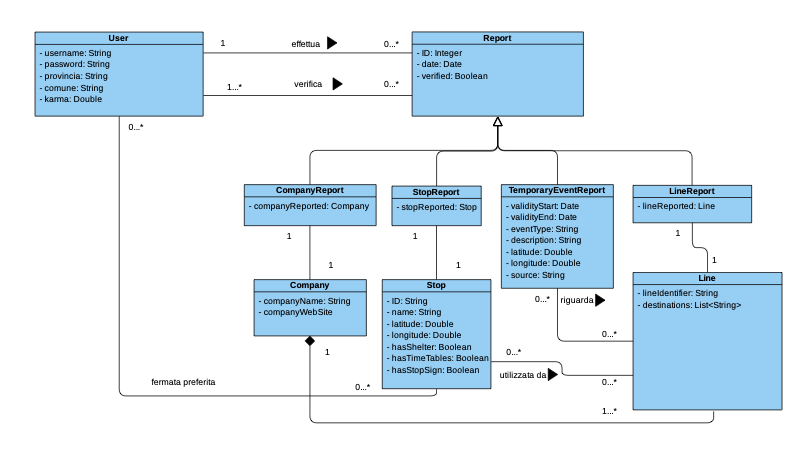
\includegraphics[width=\columnwidth]{ClassDiagram-cut}
            \caption{Il Class Diagram del Server}
            \label{fig: Il Class Diagram del Server}
        \end{figure}

    \subsection{Accessibilità delle API dall'esterno}
        Spring mette a disposizione il meccanismo dei \textbf{Controller}, che normalmente è inquadrato nel contesto di un'architettura MVC, anche se nel caso di ShallWeGo non vi è necessità di andare a creare un'applicazione di web che renda necessaria l'implementazione di tale pattern architetturale. Di conseguenza, essendo la parte che riguarda l'interfaccia utente gestita tramite un'applicazione Android, non è stata implementata nessuna parte che faccia le veci della "View" lato server. La comunicazione tra server e client avviene tramite JSON sfruttando il meccanismo delle API REST. La classe responsabile per la comunicazione con l'esterno è chiamata \textbf{Controller}, collocata nel pacchetto omonimo e decorati con l'annotazione \textbf{@RestController}. Questa annotazione permette al framework di interpretare quella classe come un Controller che accetta richieste sulla porta 8080 e all'indirizzo \url{/}. I vari metodi di quella classe che corrispondono alle diverse API esposte all'esterno sono decorati con una delle seguenti annotazioni:

        \begin{itemize}
            \item \textbf{@GetMapping("/url")} esegue il metodo annotato ogni qual volta all'indirizzo \url{/url} viene generata una richiesta di tipo \textbf{GET};
            \item \textbf{@PostMapping("/url")} esegue il metodo annotato ogni qual volta all'indirizzo \url{/url} viene generata una richiesta di tipo \textbf{POST};
            \item \textbf{@PutMapping("/url")} esegue il metodo annotato ogni qual volta all'indirizzo \url{/url} viene generata una richiesta di tipo \textbf{PUT};
            \item \textbf{@DeleteMapping("/url")} esegue il metodo annotato ogni qual volta all'indirizzo \url{/url} viene generata una richiesta di tipo \textbf{DELETE};
        \end{itemize}

    \subsection{Gestione dei dati persistenti: breve introduzione a JPA}
        Data la necessità di conservare una notevole quantità di dati (utenti, fermate, linee e così via) un approccio che prevede l'utilizzo di file è stato escluso a priori perché quasi impossibile da gestire data la complessità. Si è scelto quindi di utilizzare un database di tipo relazionale (RDBMS). Tuttavia, prevedendo il dominio applicativo numerose associazioni tra le entità, un approccio "classico" tramite \textbf{JDBC} avrebbe comunque portato ad un livello di complessità molto elevato (si pensi a dover gestire manualmente tutte le query con i vari join tra le tabelle). A questo scopo, torna molto utile sfruttare le caratteristiche di \textbf{ORM} (\textit{Object-Relational Mapping}) e, successivamente, di \textbf{JPA}, (\textit{Java Persistence API}).
        
        ORM è definito come "una tecnica di programmazione che permette l'integrazione di sistemi software che aderiscono al paradigma della programmazione orientata agli oggetti (\textbf{OOP}) con sistemi \textbf{RDBMS}".

        Uno dei principali vantaggi di ORM risiede nel contrasto della complessità di gestione della persistenza derivata dalla mancanza di compatibilità tra dati salvati all'interno di un database e oggetti in un linguaggio di programmazione, oltre che ad una sostanziale indipendenza dal \textit{vendor} che fornisce il DBMS utilizzato. \cite{wiki:orm}
        
        Il framework Spring, nello specifico, mette a disposizione una serie di API che implementano le specifiche di \textbf{JPA}. JPA è definito come "un insieme di specifiche che mette a disposizione degli sviluppatori un insieme di servizi e di strutture dati che permettono l'ORM e quindi la gestione dei dati persistenti all'interno di applicazioni Java." (\cite{jpa}). Essendo solamente una specifica, JPA necessita di un'implementazione. Quella di riferimento è \textbf{EclipseLink}, sviluppata dalla Eclipse Foundation a partire dal 2015.

        Il framework Spring, tuttavia, utilizza come implementazione delle specifiche JPA la libreria open source \textbf{Hibernate 5.5} sviluppata in partnership con l'azienda \textit{Red Hat}. 

        Per effettuare il mapping tra oggetti istanze di una classe e righe presenti in una tabella in un database, JPA si serve del concetto di \textbf{Entity}, che rappresenta un'istanza di una classe (in gergo, \textbf{POJO}, ovvero \textit{Plain Old Java Object}) che "dichiara" di poter essere salvata all'interno di un database.

        Le specifiche JPA introducono il concetto di \textbf{Configuration By Excpetion}. In questo modo, se non specificato altrimenti, le impostazioni riguardo persistenza e mapping di oggetti risulteranno essere quelle di default. Per fare un esempio concreto, in un progetto dove è previsto l'utilizzo di JPA tutte le classi Java vengono viste come tali fino a che non viene utilizzata l'annotazione Entity su una di queste. Ad esempio:

        \begin{code}
            \begin{minted}{java}
                @Entity
                public class POJO implements Serializable {
                    @Id 
                    private Integer id;

                    public POJO() {}
                }
            \end{minted}
            \caption{\textbf{File:} POJO.java}
        \end{code}
    
        Tramite questo setup è possibile rendere la classe contenuta in \textit{POJO.java} un'entity di cui è possibile effettuare la persistenza su un database.\\

        Per poter rappresentare un'Entity, un POJO deve rispettare i seguenti requisiti: (\cite{jee7})

        \begin{itemize}
            \item Essere annotata con \mintinline{java}{@javax.persistence.Entity};
            \item Avere un attributo annotato con \mintinline{java}{@javax.persistence.Id} che ne denota la chiave primaria (nel caso di chiave primaria semplice: è possibile anche avere chiavi composte, come descritto più avanti)
            \item Deve possedere un costruttore vuoto che abbia come modificatore di accesso \mintinline{java}{public} o \mintinline{java}{protected}. Sono ammessi ulteriori costruttori.
            \item Non deve essere una classe \textit{final}
            \item Non deve essere una classe interna ad un'altra classe
            \item Deve implementare l'interfaccia \mintinline{java}{Serializable}.
        \end{itemize}

        Le Entity presenti nel dominio applicativo sono le seguenti:

        \begin{itemize}
            \item \textbf{Stop}, che modella una fermata dei mezzi pubblici,
            \item \textbf{Line}, che modella una linea di trasporto pubblico,
            \item \textbf{Company}, che modella un'azienda di trasporto pubblico,
            \item \textbf{Report}, che modella il concetto di segnalazione,
            \item \textbf{LineReport}, che modella il concetto di segnalazione di una linea,
            \item \textbf{CompanyReport}, che modella il concetto di segnalazione di un'azienda,
            \item \textbf{StopReport}, che modella il concetto di segnalazione di una fermata,
            \item \textbf{TemporaryEventReport}, che modella il concetto di segnalazione di un evento temporaneo,
            \item \textbf{User}, che modella un utente registrato alla piattaforma.
        \end{itemize}

        oltre che ad altre classi "di servizio" create per mappare relazioni di tipo Many-to-Many.

        Si ponga attenzione sulla modellazione del concetto di segnalazione. Qui di seguito è mostrato lo scheletro delle classi che modellano i vari tipi di segnalazione:
        
        \begin{framed}
            \begin{code}
                \begin{minted}[autogobble]{java}
                    @Entity
                    public abstract class Report {
                        @Id 
                        private Integer Id;
                    }
                \end{minted}
                \caption{\textbf{File:} Report.java}
            \end{code}
        \end{framed}
        \begin{framed}
            \begin{code}
                \begin{minted}[autogobble]{java}
                    @Entity
                    public class StopReport extends Report {        
                        private Stop stopReported;
                    }
                \end{minted}  
                \caption{\textbf{File:} StopReport.java}
            \end{code}
        \end{framed}
        \begin{framed}
            \begin{code}
                \begin{minted}[autogobble]{java}
                    @Entity
                    public class LineReport extends Report {        
                        private Line lineReported;
                    }
                \end{minted}  
                \caption{\textbf{File:} LineReport.java}
            \end{code}
        \end{framed}
        \begin{framed}
            \begin{code}
                \begin{minted}[autogobble]{java}
                    @Entity
                    public class CompanyReport extends Report {        
                        private Company companyReported;
                    }
                \end{minted}  
                \caption{\textbf{File:} CompanyReport.java}
            \end{code}
        \end{framed}
        \begin{framed}
            \begin{code}
                \begin{minted}[autogobble]{java}
                    @Entity
                    public class TemporaryEventReport extends Report {        
                        private Date validityStart;
                        private Date validityEnd;
                        private String eventType;
                        private String description;
                        private String latitude;
                        private String longitude;
                        private String source;

                        private List<Line> affectedLines;
                    }
                \end{minted}  
                \caption{\textbf{File:} TemporaryEventReport.java}
            \end{code}
        \end{framed}
        
        Si noti l'utilizzo della keyword \mintinline{java}{extends} che segnala l'utilizzo dell'ereditarietà, un concetto tipico dei linguaggi Object-Oriented come Java e che non è modellato in nessun DBMS relazionale. Per ovviare a questo problema, JPA mette a disposizione la seguente annotazione: 

        \begin{minted}{java}
            public @interface Inheritance {
                InheritanceType strategy() default SINGLE_TABLE;
            }
        \end{minted}

        Quest'annotazione, attraverso il campo \textit{strategy} permette di stabilire con che strategia effettuare il mapping di una gerarchia.

        I valori che \textit{strategy} può assumere sono i seguenti: (\cite{jee7})

        \begin{itemize}
            \item \detokenize{SINGLE_TABLE}, che crea una sola tabella all'interno del database che rappresenta l'intera gerarchia e che per disambiguare tra i vari tipi delle sottoclassi usa un attributo chiamato "DTYPE" che assume come valore il nome della sottoclasse di un determinato elemento della tabella. Questa strategia, in virtù della configuration by exception è quella utilizzata di default in assenza dell'annotazione.
            \item \detokenize{TABLE_PER_CLASS}, che crea una tabella all'interno del database per ogni sottoclasse in una strategia.
            \item \detokenize{JOINED}, che colloca gli attributi che compaiono esclusivamente nelle sottoclassi della gerarchia in altre tabelle, una per membro della gerarchia.
        \end{itemize}

        In ShallWeGo, la strategia utilizzata è quella \detokenize{SINGLE_TABLE} poiché si è preferito non aumentare la complessità dello schema.

        Per permettere l'esecuzione delle query di inserimento, retrival ed eliminazione delle informazioni, Spring mette a disposizione il meccanismo delle \textbf{Repository}. L'obiettivo delle Repository Spring è "quello di ridurre la quantità di codice \textit{boilerplate} necessario per implementare il layer di accesso ai dati per diversi tipi di entità persistenti.".

        La creazione delle Repositories è demandata al programmatore che può crearne una creando un'\textbf{interfaccia} che estende la classe \mintinline{java}{CrudRepository<T, ID>} oppure \\ \mintinline{java}{JpaRepository<T, ID>}.

        \begin{itemize}
            \item \textbf{T} indica la classe dell'Entity a cui la repository si riferisce;
            \item ID indica la classe della \textbf{chiave primaria} di T
        \end{itemize}

        La particolarità delle Repositories di Spring è sostanzialmente quella di poter andare a creare delle query semplicemente andando ad aggiungere un metodo all'interfaccia appena creata. Ad esempio, se nel caso di un'Entity si ha necessità di effettuare query basandosi su due attributi (X ed Y), allora sarà sufficiente aggiungere questo metodo all'interfaccia associata all'Entity:

        \begin{code}
            \begin{minted}[autogobble]{java}
                public interface EntityRepository extends
                 JpaRepository<Entity, Integer> {
                    public List<Entity> findByXAndY(String X, String Y);
                }
            \end{minted}
            \caption{Esempio di Repository con custom query}
        \end{code}

        In ShallWeGo, le seguenti Repository sono state utilizzate:

        \begin{itemize}
            \item \textbf{CompanyRepository} che permette di effettuare query riguardanti l'Entity \textbf{Company}
            \item \textbf{LineRepository} che permette di effettuare query riguardanti l'Entity \textbf{Line}
            \item \textbf{ReportRepository} che permette di effettuare query riguardanti l'Entity \textbf{Report}
            \item \textbf{StopRepository} che permette di effettuare query riguardanti l'Entity \textbf{Stop}
            \item \textbf{TemporaryEventReportRepository} che permette di effettuare query riguardanti l'Entity \textbf{TemporaryEventReport}
            \item \textbf{UserRepository} che permette di effettuare query riguardanti l'Entity \textbf{User}
        \end{itemize}

        Nel caso particolare di \textbf{UserRepository}, si può notare come sia stata introdotta una query per recuperare dal database tutti gli utenti che operano in una determinata provincia. Questo si è reso necessario per il funzionamento dell'algoritmo di assegnazione dei verificatori di una segnalazione:

        \begin{code}
            \begin{minted}[autogobble]{java}
                public interface UserRepository extends JpaRepository<User, String> {
                    List<User> findByProvincia(String provincia);
                }
            \end{minted}
            \caption{\textbf{File:} UserRepository.java}
        \end{code}
        

    \subsection{Mappe e Dati Geografici: OpenStreetMap e Nominatim}
        OpenStreetMap è un \textbf{WebGIS} lanciato nel 2004 che si propone come alternativa open source ai servizi commerciali che forniscono mappe o dati geografici in generale (si pensi ad esempio ai nomi delle strade oppure delle attività commerciali). Adotta un approccio \textbf{community-driven}: di conseguenza, i dati sono aggiornati periodicamente da parte di utenti che aderiscono al progetto. Questi dati sono consultabili tramite l'interfaccia principale del servizio, disponibile all'indirizzo \url{https://www.openstreetmap.org/}. All'interno di questa pagina è presente, come nella maggior parte dei servizi di questo tipo, una casella di ricerca che permette di cercare indirizzi o punti di interesse. La funzionalità di ricerca è implementata sfruttando il servizio \textbf{Nominatim}, già accennato in precedenza.
        Nominatim consiste in un sistema \textbf{geocoding} open source scritto in PHP e sviluppato con il patrocinio dello stesso progetto OpenStreetMap. Esso permette di effettuare ricerche di dati geografici presenti all'interno di un database PostgreSQL a partire da un insieme di parole chiave e, allo stesso modo, di ottenere suddetti dati a partire da una coppia di coordinate (Latitudine, Longitudine). Il progetto Nominatim viene inoltre usato anche dalla stessa piattaforma OpenStreetMap per fornire la funzionalità di ricerca all'interno della propria interfaccia web.
        Il server Nominatim, nel caso specifico della piattaforma, è stato utilizzato principalmente per ottenere due tipologie di informazioni:
        \begin{itemize}
            \item A partire dal nome di un comune e dalla sua provincia, una coppia di coordinate (Latitudine, Longitudine) che ne rappresenti la posizione approssimativa al fine di computare la fitness di un individuo nel contesto dell'algoritmo genetico
            \item Per fornire, oltre alla posizione in termini di coordinate, anche un indirizzo approssimativo (e quindi un nome mnemonico) per una segnalazione indicata come \textit{evento temporaneo}. In questo caso, si parla di \textit{reverse geocoding}
        \end{itemize}
        Uno dei principali vantaggi di questa piattaforma consiste nella possibilità da parte di un utente di installare la propria istanza del server, importando all'interno di un database una serie di dati provenienti da diverse fonti. 
        La strada del self-hosting è quella che preferita nel caso di ShallWeGo, poiché nonostante sia disponibile un endpoint pubblico a cui possono essere indirizzate delle richieste, disponibile alla pagina \url{https://nominatim.openstreetmap.org/} esso impone una restrizione di esattamente una interrogazione al secondo, pena il \textit{ban} dell'indirizzo IP sorgente dall'utilizzo del servizio. 
        Nel caso particolare di ShallWeGo è stata utilizzata la versione 3.7.2 del software, installata su una macchina che esegue il Sistema Operativo Arch Linux e che utilizza \textit{Apache httpd} come server web per esporre il servizio in rete.

        I servizi di Nominatim sono accessibili sostanzialmente in due modi: 
        
        \begin{itemize}
            \item Tramite un'interfaccia utente di debug che include sia una casella di ricerca, sia una mappa dove visualizzare i risultati
            \item Tramite API REST, che permettono l'output testuale dei risultati in diversi formati (tipicamente JSON e XML).
        \end{itemize}

        Avendo necessità di utilizzare il risultato all'interno di un'altra componente, è stata reputata non essenziale la configurazione della GUI di Nominatim: in ShallWeGo viene usata solamente la sua interfaccia che prevede output testuale.

        In particolare, di seguito sono descritti i servizi di Nominatim utilizzati dalla piattaforma per i suoi scopi:

        \begin{itemize}
            \item \textbf{/search}: il servizio principale e quello più usato. Permette di ottenere risultati in termini di dati OSM (e quindi anche le coordinate geografiche corrispondenti) di un luogo a partire da un insieme di parole chiave. Queste ultime possono essere specificate tramite il parametro \textbf{q}. Ad esempio, la query associata a  \url{http://nominatim.openstreetmap.org/search/?q=Universita Degli Studi di Salerno Fisciano&format=json} permette di ottenere informazioni sul campus di Fisciano dell'Università degli Studi di Salerno in formato JSON (Si veda la figura 4.1);
            \item \textbf{/reverse}: permette di ottenere approssimativamente l'indirizzo associato a delle coordinate geografiche specificate tramite i parametri \textbf{lat} e \textbf{lon}, che rappresentano rispettivamente la latitudine e la longitudine del luogo. Ad esempio, la query associata a \url{http://nominatim.openstreetmap.org/reverse/?lat=40.774283&lon=14.790868&format=json} permette di ottenere le informazioni associate alle coordinate (40.774283, 14.790868) in formato JSON. (Si veda la figura 4.2)
        \end{itemize}

        \begin{figure}[htp]
            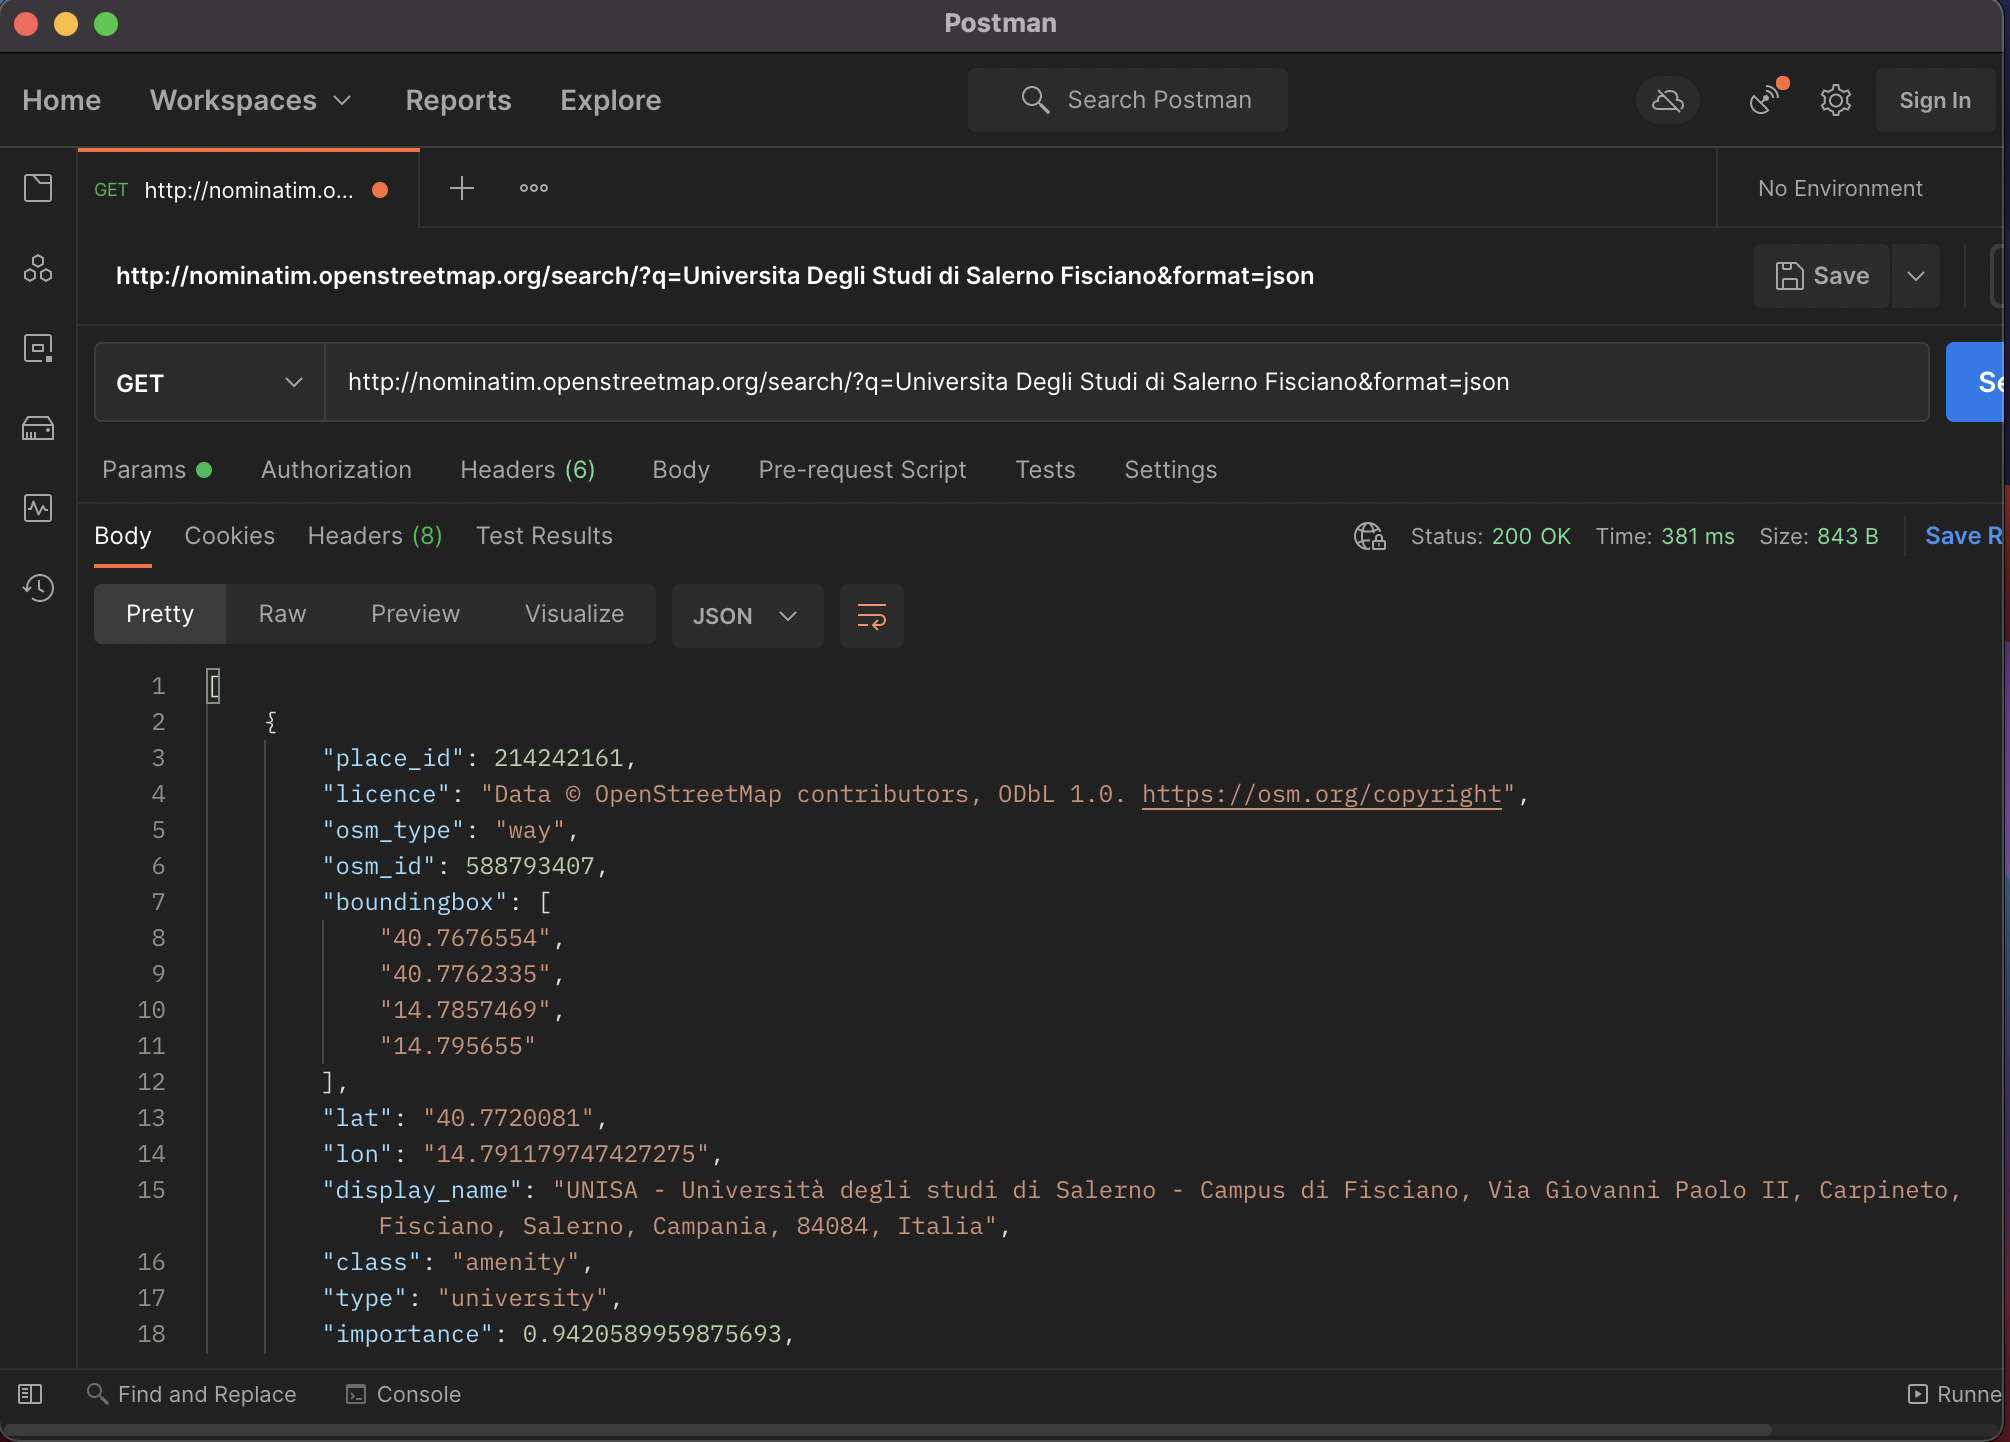
\includegraphics[width=\columnwidth]{search}
            \caption{Search}
            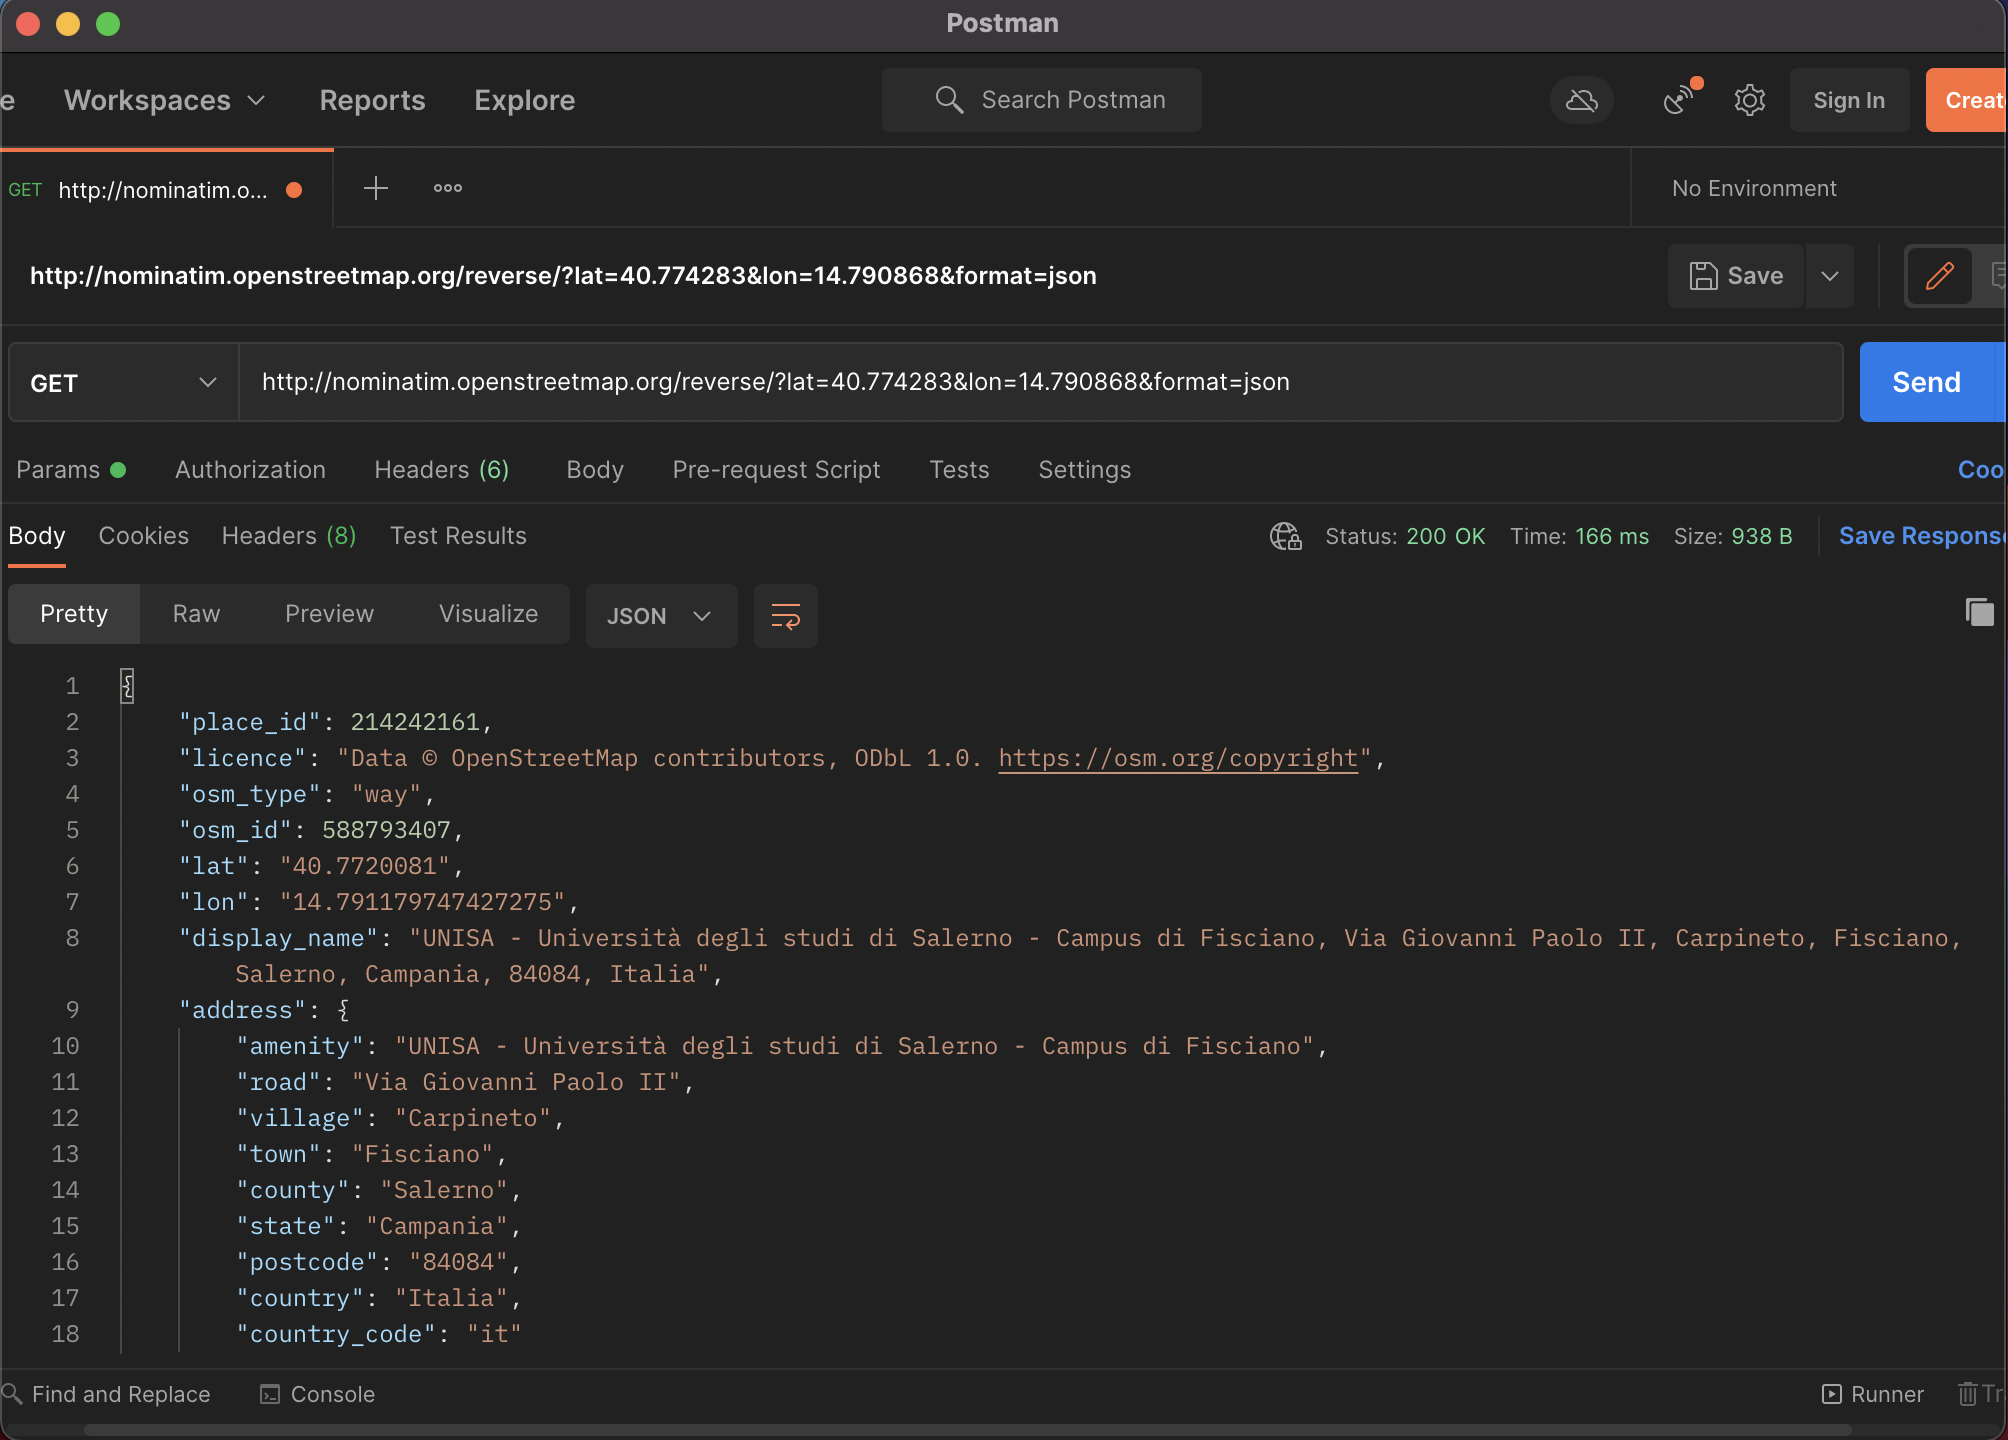
\includegraphics[width=\columnwidth]{reverse}
            \caption{Reverse}
        \end{figure}


        \newpage
        \subsubsection{Fonte dei dati utilizzati}
            Nominatim di per sé risulta essere solamente un servizio che permette di effettuare geocoding a partire da un dataset ma non ne fornisce nessuno out of the box. È stato quindi necessraio ottenere questi dati da entità terze. Un progetto che mette a disposizione pubblicamente questo tipo dei dati è chiamato Geofabrik, che ospita sui suoi server pacchetti organizzati per Stato o per Continente. Il formato di questi pacchetti risulta essere $.osm.pbf$, che è possibile importare all'interno di Nominatim attraverso un applicativo chiamato \textbf{osm2pgsql}. Quest'applicativo permette di importare dati organizzati secondo lo standard di OpenStreetMap all'interno di un database PostgreSQL/PostGIS. \\
            
        \newpage
        \section{ShallWeGo: Il client}
            Dopo aver analizzato in dettaglio la Java Application che contiene la logica applicativa di ShallWeGo ed aver descritto il funzionamento del Server di Geocoding si passa ora all'analisi del client della piattaforma.
            Il client messo a disposizione dalla piattaforma consiste in un'applicazione Android sviluppata usando il linguaggio Java.

        \subsection{Breve introduzione allo sviluppo Android}
            La piattaforma Android è storicamente molto aperta allo sviluppo di applicativi di terze parti. Già a partire dalla versione 1.0 (rilasciata nel 2009), Google si è impegnata a fornire un'API completa e semplice da usare per facilitare sia lo sviluppo di app sia il funzionamento di nuove versioni del sistema operativo stesso su un determinato hardware (tramite il progetto \textbf{AOSP}, ovvero \textit{Android Open Source Project})

            Un'applicazione Android, astraendosi dal funzionamento a basso livello del sistema operativo (il cui \textit{kernel}) si basa su Linux, consiste soprattutto in \textbf{Activity}.

            Un'Activity, secondo la documentazione ufficiale, è un "task singolo e specifico che l'utente può effettuare" \cite{AndroidDoc}. Quasi tutte le Activity interagiscono con l'utente e, tramite operazioni normalmente trasparenti allo sviluppatore, si occupano della composizione delle finestre, che saranno poi utilizzate per mostrare la User Interface creata da chi sviluppa l'applicazione (che si specifica usando un file XML che è strettamente legato ad un'Activity).

            Fino al 2019, Java ha rappresentato il linguaggio di programmazione principale per lo sviluppo di app Android. Alla conferenza Google I/O di quello stesso anno è stato annunciato l'impiego di \textbf{Kotlin} come linguaggio primario. Uno dei vantaggi di Kotlin è rappresentato dalla sua sintassi più concisa rispetto a quella di Java mantenendo comunque l'\textbf{interoperabilità} con quest'ultimo.
        
        \subsection{Activity presenti nell'applicazione}
            Come accennato in precedenza, le app Android sono costituite perlopiù da Activity, che permettono l'interazione con l'utente.

            In ShallWeGo ne sono presenti 18. Ognuna di queste rappresenta una feature specifica della piattaforma.

            Nello specifico:

            \begin{itemize}
                \item \textbf{IntroSlideShow}: fornisce una presentazione ed una panoramica sullo scopo e sul funzionamento dell'applicazione. È utilizzata inoltre per concedere i permessi per l'utilizzo dei servizi di geolocalizzazione;
                \item \textbf{RegisterActivity}: permette la registrazione di un'utente alla piattaforma;
                \item \textbf{LoginActivity}: permette il login di un utente registrato alla piattaforma;
                \item \textbf{MainActivity}: l'Activity principale di qualsiasi app Android e la prima ad essere avviata quando l'utente apre l'app. Contiene una mappa dove sono presenti, sotto forma di marker, gli oggetti di interesse della piattaforma (fermate, corse ed eventi temporanei);
                \item \textbf{AlertsNearby}: permette all'utente di visualizzare gli eventi temporanei più vicini alla propria zona;
                \item \textbf{FavoriteStops}: permette all'utente di accedere velocemente alle fermate che ha aggiunto all'elenco delle sue preferite;
                \item \textbf{StopDetails}: permette all'utente di accedere alla pagina dei dettagli di una fermata specifica;
                \item \textbf{EventDetails}: permette all'utente di consultare i dettagli di un evento temporaneo;
                \item \textbf{CompanyReportActivity}: permette all'utente di effettuare la segnalazione di un'azienda di trasporto;
                \item \textbf{LineReportActivity}: permette all'utente di effettuare la segnalazione di una linea;
                \item \textbf{StopReportActivity}: permette all'utente di effettuare la segnalazione di una fermata e di specificare le linee che la utilizzano;
                \item \textbf{TemporaryEventReportActivity}: permette all'utente di effettuare la segnalazione di un evento temporaneo ed eventualmente di specificare le linee coinvolte;
                \item \textbf{MyReportsActivity}: permette all'utente di visualizzare tutte le segnalazioni che ha effettuato nel tempo;
                \item \textbf{NewRideActivity}: permette all'utente di comunicare la propria posizione nell'ambito di una corsa espletata da una determinata linea. Permette di comunicarne anche l'affollamento e lo stato del mezzo in termini di presenza di aria condizionata e di macchina validatrice dei titoli di viaggio.
                \item \textbf{VerifyReports}: permette all'utente di visualizzare tutte le segnalazioni non ancora approvate a cui è stato assegnato in qualità di \textit{verificatore};
                \item \textbf{VerifyCompanyReport}: permette al \textit{verificatore} di fornire il proprio voto sulla segnalazione di un'azienda di trasporto;
                \item \textbf{VerifyLineReport}: permette al \textit{verificatore} di fornire il proprio voto sulla segnalazione di una linea espletata da un'azienda di trasporto;
                \item \textbf{VerifyStopReport}: permette al \textit{verificatore} di fornire il proprio voto sulla segnalazione di una fermata;
            \end{itemize}
        
            \subsection{Librerie di terze parti utilizzate nell'applicazione}
                Dal 2013, i progetti Android utilizzano il toolkit \textbf{Gradle}. Gradle consiste in una serie di utility eseguite sulla JVM che permettono la semplificazione e l'automazione del processo di \textit{build} delle applicazioni. Uno dei compiti principali di un build manager come Gradle consiste nella gestione delle dipendenze e dei moduli di terze parti che possono essere inclusi in un'applicazione. In un progetto Android, solitamente, le dipendenze vanno specificate nel file \textit{build.gradle} dell'applicazione.

                Durante lo sviluppo di ShallWeGo, per fornire tutte le funzionalità indicate in precedenza, si è fatto uso di diverse librerie di terze parti, il cui funzionamento ed impiego nella piattaforma verrà descritto di seguito.

                \subsubsection{OsmDroid: un'alternativa \textit{free} a Google Maps}
                    Come accennato nell'introduzione, l'applicazione fa largo uso di mappe e dati geografici in generale. Si è parlato di come applicativi e librerie libere ed open-source potessero andare a risolvere il problema della dipendenza da servizi come le API di Google Maps, che prevedono un costo superata una certa soglia di utilizzo periodica. Anche l'integrazione di una mappa all'interno di un'Activity (che accade molto spesso nel contesto di ShallWeGo), se si opta per il servizio messo a disposizione da Google Maps, richiede il possesso di un'\textbf{API key} che permette di identificare univocamente la fonte delle richieste e tenere sotto controllo le soglie di utilizzo, eventualmente procedendo ad addebiti nel caso di sforamento. Per far fronte a questa problematica (che si fa più urgente man mano che l'utilizzo della piattaforma aumenta) è stata impiegata la libreria \textbf{OsmDroid}, che si propone come un'alternativa completa e gratuita alle API di Google Maps per l'integrazione di mappe all'interno di applicazioni Android. I dati della mappa fornita da questa libreria provengono dal progetto OpenStreetMap, di cui si è discusso precedentemente. Il codice sorgente e la documentazione della libreria sono disponibili interamente su GitHub all'indirizzo \url{https://github.com/osmdroid/osmdroid}.

                \subsubsection{AppIntro}
                    \textbf{AppIntro} è una libreria creata dallo sviluppatore \textbf{Paolo Rotolo} la cui documentazione è disponibile su GitHub all'indirizzo \url{https://github.com/AppIntro/AppIntro}. Fornisce il supporto alla creazione, sotto forma di \textit{slides} di un'introduzione all'applicazione. Questo modulo semplifica notevolmente il processo di richiesta dei permessi, diventato più complesso dall'introduzione di Android 5.0.
                    La libreria è stata impiegata per realizzare l'activity \textbf{IntroSlideShow}.

                \subsubsection{Volley}
                    \textbf{Volley} è una libreria sviluppata da \textbf{Google} per fornire delle API da usare per svolgere task che richiedono l'interazione con la rete. L'impiego di questa libreria è stato preferito poiché la mole delle richieste da effettuare non è tale da giustificare l'utilizzo di altre librerie che Google stessa consiglia per trasferimenti di grandi moli di informazioni attraverso la rete come il \textbf{Download Manager} accessibile dalle API di Android. Il funzionamento di Volley si basa sulla presenza di una \textit{coda} di richieste (realizzata tramite la classe \mintinline{java}{RequestQueue}) alla quale possono essere aggiunte delle richieste e all'evenienza regolarne la priorità in caso di richieste multiple.
                    Dopo aver aggiunto una richiesta alla coda, Volley provvederà a spedirla in maniera \textbf{asincrona} e ad eseguire il metodo di callback \mintinline{java}{onResponse()} dal quale è possibile provvedere all'aggiornamento della UI. In ShallWeGo, la libreia è stata utilizzata in quasi tutte le Activity per realizzare l'interazione con la Java Application tramite file JSON dai quali sono estratte le informazioni necessarie per aggiornare l'interfaccia in modo corretto.
                
                \subsubsection{Gson}
                    \textbf{Gson} è una libreria anch'essa sviluppata da \textbf{Google} che permette la serializzazione e la deserializzazione di informazioni da ed in stringhe JSON. La libreria mette a disposizione le classi \mintinline{java}{JsonObject} e \mintinline{java}{JsonArray} che modellano rispettivamente un oggetto ed un array di oggetti JSON e che permettono di accedere (tramite il metodo \mintinline{java}{get()}) in maniera strutturata ai vari campi della stringa di cui viene effettuato il parsing. Allo stesso modo, le classi \mintinline{java}{JsonObject} e \mintinline{java}{JsonArray} permettono di organizzare dei dati che possano essere convertiti correttamente in una stringa JSON. Insieme a Volley, questa è una delle librerie fondamentali che permettono il corretto funzionamento della comunicazione con le API esposte dalla Java Application. Dunque, questa libreria è stata usata ogni qual volta è risultato necessario comunicare col server.

                \subsubsection{Material Components}
                    \textbf{Material Components} è una libreria sviluppata da Google che fornisce l'implementazione (sia dal punto di vista di classi Java sia dal punto di vista di elementi XML pronti da inserire nei file di layout) di una serie di componenti grafiche tipiche del \textbf{Material Design}. Il Material Design è un sistema di design introdotto da Google stessa nel 2014 con la versione 5.0 di Android ed in continua evoluzione anche oggi. Il layout delle Activity di ShallWeGo è realizzato usando quasi esclusivamente queste componenti.
                
                \subsubsection{SpeedDial}
                    \textbf{SpeedDial} è una libreria creata dallo sviluppatore \textbf{Roberto Leinardi} la cui documentazione è disponibile all'indirizzo \url{https://github.com/leinardi/FloatingActionButtonSpeedDial}. Fornisce un'implementazione concreta di un \textbf{Floating Action Button} (o \textbf{FAB}) seguendo le specifiche descritte alla pagina \url{https://material.io/components/buttons-floating-action-button#types-of-transitions}. Un Floating Action Button è solitamente un pulsante posizionato in vari punti del layout di un'Activity che permette di "richiamare" l'attenzione dell'utente, indicandogli il punto in cui è possibile compiere le azioni principali che quella determinata Activity mette a disposizione, che verranno mostrate alla pressione del FAB (\textit{Speed Dial}). La libreria sopracitata permette proprio questo comportamento. In ShallWeGo, questa libreria è utilizzata in accoppiata col FAB presente nella MainActivity che, una volta premuto, offre l'opportunità di eseguire i seguenti task:

                    \begin{itemize}
                        \item Riposizionare la mappa in corrispondenza della posizione attuale dell'utente;
                        \item Effettuare una segnalazione nella posizione attuale dell'utente;
                        \item Cominciare il tracciamento in diretta di una corsa. (Il funzionamento di questo aspetto viene trattato in dettaglio nella sezione successiva).
                    \end{itemize}

                    Le figure 4.4 e 4.5 mostrano rispettivamente il FAB presente nella MainActivity e lo Speed Dial ad esso associato.
                    \\
                    \\
                    \begin{figure}[ht]
                        \begin{minipage}[b]{0.45\linewidth}
                          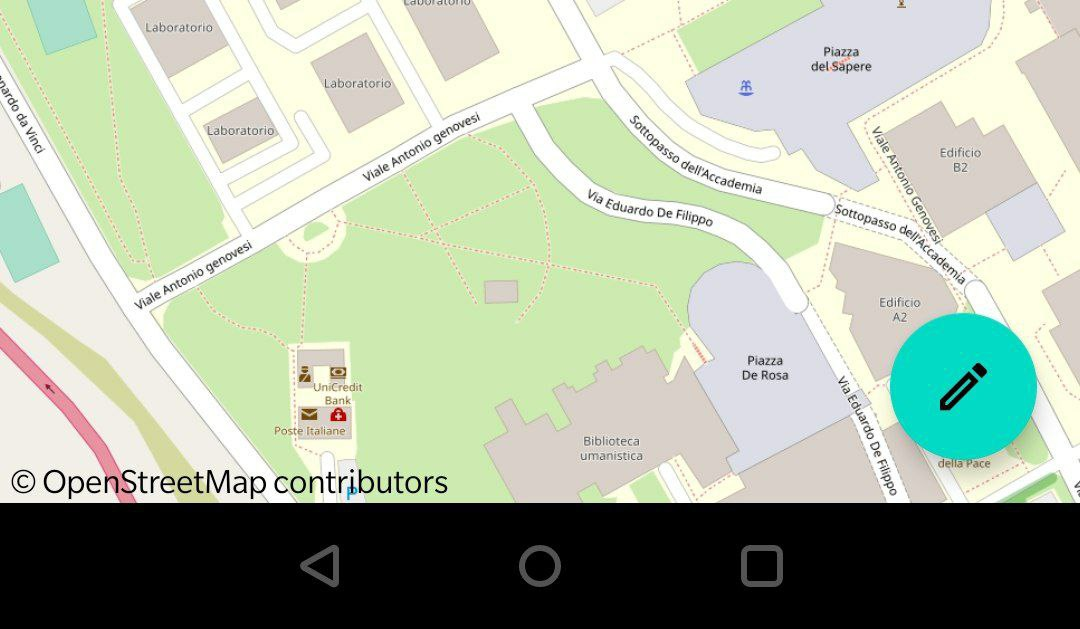
\includegraphics[width=1.0\textwidth]{capitolo4/figure/fab.jpg}
                            \centering
                          \caption{FAB nella Main Activity}
                          \label{fig:FAB nella Main Activity}
                        \end{minipage}
                        \quad
                        \begin{minipage}[b]{0.45\linewidth}
                           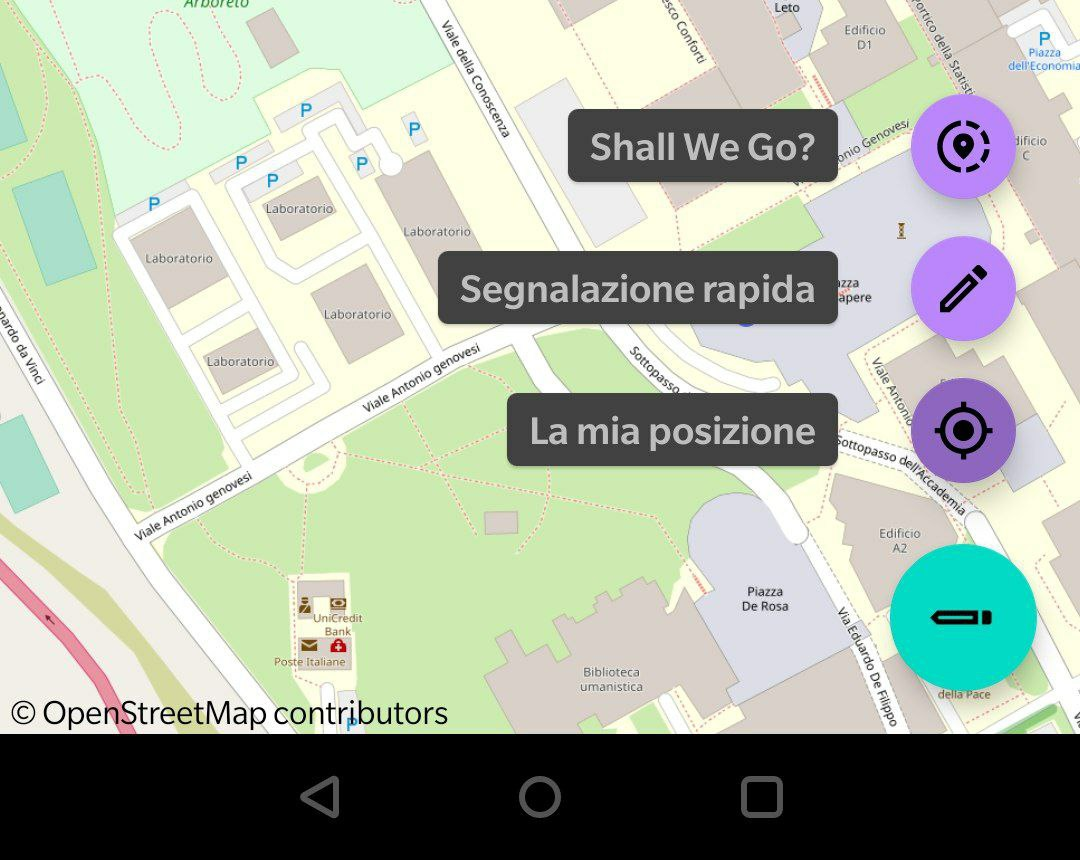
\includegraphics[width=1.0\textwidth]{capitolo4/figure/speeddial.jpg}
                           \centering
                         \caption{Speed Dial associato al FAB}
                         \label{fig:Speed Dial associato al FAB}
                       \end{minipage}
                       \end{figure}
                    \newpage

        \subsection{Il tracciamento in diretta delle corse: overview sui servizi di Android}
            Una delle funzionalità di ShallWeGo permette all'utente collegato alla piattaforma di mettere a disposizione degli altri utenti la propria posizione all'interno di una corsa espletata da una linea di trasporto pubblico.
            Realizzare una funzionalità del genere implica dover recuperare ad intervalli regolari la posizione esatta del dispositivo che l'utente sta utilizzando ed inviare una richiesta alla Java Application che si occuperà di aggiornare i dati in suo possesso.
            
            \subsubsection{Services}
                Per task di questo genere, Android mette a disposizione dello sviluppatore una serie di API che ne permettono un'implementazione facile e veloce: i \textbf{Servizi}.

                Secondo la documentazione ufficiale, un Servizio è "una componente applicativa utile ad eseguire un task dalla durata prolungata, che può continuare anche se l'utente passa ad un'altra applicazione" (\cite{AndroidDocService}).

                In Android esistono due tipi di Servizi: 

                \begin{itemize}
                    \item \textbf{Foreground};
                    \item \textbf{Background} 
                \end{itemize}

                Un \textbf{Background Service} è un servizio che permette di svolgere task, come suggerisce la denominazione, in background (ovvero anche quando l'Activity che l'ha fatto partire non è visibile a schermo). L'utente solitamente non è tenuto a sapere se e quando questo tipo di servizi sia in esecuzione. Quest'ultimo aspetto potrebbe portare a problemi di privacy o sicurezza in caso di impiego da parte di applicazioni malevole o anche di prestazioni nel caso in cui il task da svolgere sia pesante in termini di utilizzo di risorse. Per questa ragione, dalla versione 26 delle API (ovvero a partire dalla versione 8.0 di Android), sono state introdotte delle limitazioni ai servizi in background. \\
                Se un'applicazione non è più visibile a schermo (nella maggior parte die casi, quando l'utente torna alla \textit{home} sul proprio device), essa è considerata essere in background. Quando un'applicazione è in background, a partire da Android 8.0 il sistema le concede un intervallo di tempo prestabilito, scaduto il quale il sistema \textbf{termina tutti servizi in background dell'applicazione}. Data la natura della feature che deve essere realizzata, questo comportamento risulta non accettabile (e dunque non è stato possibile implementarla tramite un background service).
                
                Un \textbf{Foreground Service}, invece è "un servizio che permette di svolgere task di cui l'utente dovrebbe essere informato" (\cite{AndroidDocForeground}). Per funzionare, un Foreground Service deve obbligatoriamente mostrare una notifica all'utente nella barra di stato, appunto per permettere all'utente di rendersi conto della presenza di quel task in esecuzione. Applicazioni che fanno uso di Foreground Service sono per esempio i player musicali, che mostrano come notifica la canzone attualmente in riproduzione. Contrariamente a quanto ci si aspetterebbe dalla denominazione, i Foreground Service \textbf{possono essere in esecuzione anche in background}, a patto che siano stati avviati dall'utente o da un'Activity in esecuzione in quel momento. Il vantaggio principale di utilizzare un Foreground Service sta nel fatto che, mentre quest'ultimo risulta in esecuzione, l'applicazione che lo ospita non viene considerata in background ed il Sistema non la termina per recuperare risorse. Inoltre, da Android 10 (API 29) in su è stata rimossa la possibilità di concedere il permesso alla geolocalizzazione anche in background, demandando all'utente il compito di concederlo direttamente dalle impostazioni di sistema. Alla luce di quanto si è detto, l'utilizzo di un foreground service è un buon modo per evitare la gestione di questa limitazione. In ShallWeGo, infatti, si è deciso di utilizzare quest'approccio per la gestione degli aggiornamenti sulla posizione.

                Al di là della tipologia di servizio, ognuno di questi deve essere dichiarato all'interno del \textit{Manifest} dell'Applicazione, che può essere visto come un descrittore di ciò che l'app contiene. Nel Manifest vanno specificate tutte le activity e tutti i servizi presenti.

                \subsubsection{LiveTracking}
                    \textbf{LiveTracking} è il Foreground Service che si occupa degli aggiornamenti sulla posizione di una corsa tracciata da un utente.

                    \begin{center}
                        \begin{code}
                            \begin{minted}{xml}
                <service
                    android:name=".LiveTracking"
                    android:foregroundServiceType="location"
                    android:enabled="true"
                    android:exported="true"
                    android:stopWithTask="true">
                </service>
                            \end{minted}
                            \caption{Snipped di AndroidManifest.xml che contiene la dichiarazione del Servizio}
                        \end{code}
                    \end{center}
    
                    Si noti l'attributo \mintinline{xml}{android:foregroundServiceType}. È un attributo specifico dei Foreground Services che ne determina il tipo. Se non lo si specifica, quando il Servizio sta per essere avviato, il Sistema Operativo solleva un'eccezione.

                    L'attributo \mintinline{xml}{android:stopWithTask} permette di specificare se il servizio debba essere arrestato quando l'utente chiude dal multitasking o termina l'applicazione (se posto a \mintinline{java}{true}) o meno (se posto a \mintinline{java}{false}). Si è scelto di utilizzare quest'opzione per dare all'utente un modo veloce per terminare la propria corsa in modo veloce senza passare per l'applicazione (o in caso di possibili malfunzionamenti).


                    \subsubsection{Avvio del Servizio}
                        Quando un utente decide di condividere la propria posizione allo scopo di eseguire il tracciamento in diretta di una corsa, è invitato, nell'Activity \textbf{NewRide} a compilare una serie di campi che indicano lo stato della corsa e la linea che la espleta. A questo punto, la \textbf{MainActivity} provvede ad inviare i dati alla Java Application tramite una chiamata all'API \mintinline{java}{initRide}, che conterrà tutti i dettagli sulla corsa. Il server risponderà con l'\textbf{ID} della corsa appena comunicata. Alla ricezione di questa risposta, la MainActivity provvede ad avviare il servizio tramite il metodo \mintinline{java}{startForegroundService(Intent intent)}. Il parametro \mintinline{java}{intent} del metodo rappresenta "una descrizione astratta di un'operazione da svolgere" (\cite{AndroidIntent}). In generale, gli Intent vengono utilizzati per scambiare dati di piccola entità tra le varie Activity all'atto del loro avvio, ma anche per comunicare ad un Sevizio che si intende avviarlo o comunque comunicargli qualcosa, come nel caso di LiveTracking, mediante il metodo \mintinline{java}{setAction()}, che va a specificare l'azione che si intende far intraprendere al servizio, che sarà interpretata da quest'ultimo tramite la sovrascrittura del metodo \mintinline{java}{onStartCommand()}. Per l'avvio del Servizio, l'Action dell'intent inviato tramite \mintinline{java}{startForegroundService(Intent intent)} risulta essere  
                        \texttt{$START\_SERVICE$}.
                    \subsubsection{Aggiornamenti periodici: FusedLocation e LocationUpdates}
                        Per ottenere informazioni sulla geolocalizzazione, il servizio fa uso dell'API di Google denominata \textbf{FusedLocation}, presente nella libreria dei \textbf{Google Play Services} dedicata proprio alla gestione della posizione.
                        FusedLocation è "un'API di localizzazione che combina intelligentemente diverse fonti (GPS o Rete Mobile) per mettere a disposizione le informazioni di geolocalizzazione alle app". (\cite{PlayServicesFusedLocation}).

                        La particolarità dell'API FusedLocation consiste nel supporto ai \textbf{Location Updates}, tramite i quali è possibile ottenere aggiornamenti continui sulla posizione del dispositivo specificandone la precisione e l'intervallo col quale ottenere un nuova posizione.
                        Nello specifico, per poter iniziare a ricevere aggiornamenti continui sulla posizione, è stato necessario ottenere un'istanza del \mintinline{java}{FusedLocationProviderClient} tramite il metodo 
                        \mintinline{java}{getFusedLocationProviderClient}.
                        Una volta ottenuto quest'oggetto è necessario andare a creare una nuova \textbf{LocationRequest}, tramite il metodo statico \mintinline{java}{LocationRequest.create()}. Questo oggetto serve a determinare i vari parametri della richiesta, come la priorità che le verrà riservata e l'intervallo (in millisecondi) tra una richiesta e l'altra.
                        Come ultimo step, è necessario definire un \textbf{metodo di callback}, ovvero un metodo che verrà eseguito in corrispondenza del risultato di una singola richiesta. Il metodo di callback è definito tramite l'implementazione di una \textbf{classe anonima} chiamata appunto \mintinline{java}{LocationCallback}.\\
                        Il metodo di callback implementato nel servizio LiveTracking si occupa, una volta disponibile una posizione, della comunicazione di quest'ultima col server. 
                        La Java Application espone un'API chiamata \mintinline{java}{updateRideLocation}, che permette proprio di portare a termine questo task.
                        Il processo avviene iterativamente grazie proprio al meccanismo dei Location Updates. 
                        
                        
                        \subsubsection{Termine del Servizio}
                            Il processo di comunicazione della posizione in diretta al server termina nello stesso esatto momento in cui termina il Servizio.
                            Il Servizio può terminare in due modi:

                            \begin{itemize}
                                \item L'utente preme il \textbf{pulsante di terminazione} sulla notifica nella barra delle notifiche che comunica l'esecuzione del processo.
                                \item L'utente chiude l'applicazione e la rimuove dalle app recenti.
                            \end{itemize}

                            Quando una delle due condizioni si verifica, al servizio è passato un \textbf{Intent} che contiene l'azione \texttt{$STOP\_SERVICE$}. In questo caso, il client provvede a contattare l'API \mintinline{java}{terminateRide}, che consente al server di cancellare la corsa dall'elenco di quelle in esecuzione.
                        
                            \subsubsection{Comunicazione tra Servizio ed Activity}
                                LiveTracking si occupa nello specifico di aggiornare i dati sulla geolocalizzazione e del loro invio al server ma non si occupa (e non può occuparsi) di rendere coerente l'Interfaccia Utente dei cambiamenti che raccoglie. Sulla mappa presente nella MainActivity è presente, quando il tracciamento in diretta è attivo, un Marker che rappresenta la posizione in un determinato momento di quella specifica corsa. All'aggiornarsi della posizione, anche quella del Marker deve essere aggiornata: sorge quindi la necessità di mettere in comunicazione in qualche modo il Servizio e la MainActivity. Questo problema può essere risolto mediante il meccanismo dei \textbf{Broadcast}. Un Broadcast è un tipo specifico di messaggio che viene inviato da un'app o dal Sistema Operativo quando avviene un evento considerato di interesse. Questo meccanismo funziona anche tra più componenti della stessa applicazione (ed in questo caso non è presente nemmeno l'overhead introdotto dalla \textit{Inter-Process Communication}). Quest'ultimo apsetto, unito all'immediatezza con la quale avviene questa comunicazione, ha fatto sì che la scelta per l'implementazione tra LiveTracking e la MainActivity ricadesse proprio su questo meccanismo. Nello specifico: 
                                \begin{itemize}
                                    \item All'interno del servizio, viene sfruttato il metodo \mintinline{java}{sendBroadcast(Intent intent)}, che permette di inviare un broadcast che ha come \textit{action} quella specificata da \mintinline{java}{intent}.
                                    \item All'interno della MainActivity è presente un \mintinline{java}{LocalBroadcastReceiver} che, tramite il metodo \mintinline{java}{onRecevive()} permette di intercettare messaggi Broadcast. All'interno di questo metodo è implementata la logica per aggiornare la UI sia quando è presente un nuovo aggiornamento della posizione da parte del provider FusedLocation sia quando il Servizio termina e il Marker che simboleggia la corsa che l'utente stava tracciando deve essere rimosso dalla mappa.
                                \end{itemize}

                                Per permettere il funzionamento dei receivers è necessario \textbf{registrare} il ricevitore, tramite il metodo
                                \mintinline{java}{registerReceiver(BroadcastReceviver receiver, IntentFilter filter)}.
                                Il secondo parametro del metodo, filter, è necessario per specificare quali tipi di messaggi broadcast dovrebbero far attivare il ricevitore. È possibile specificarli tramite il metodo \mintinline{java}{setAction(String action)} della classe \mintinline{java}{IntentFilter}, dove \textit{action} corrisponde al tipo di messaggio che si vuole aggiungere al filtro.              